\section{Sprint 3}

\subsection{Sprint planning}
	In sprint 3 the group planned on implementing the final requirements with high priority, as well as most of the requirements with medium priority. This is the second to last sprint, and it is important that in the last sprint the  only remaining requirements are medium to low requirements, so that time can also be spent fixing bugs and make the game work properly on iOS. The goal for this sprint will be to get a fully playable game, with only minor requirements missing.

	A usability test will be carried out in the last week of the sprint to discover potential bugs or errors we have yet to discover, as well as ideas for improvements that may be implemented in the next sprint.

	Concerning the report, we plan to finish the content up until this sprint.

\subsection{Duration and workload}
	
	{\bf Duration:} 14.10 - 27.10 (2 weeks)\\
	{\bf Workload:} This is the list with hours spent (the whole grup) on the project in this sprint.
	\begin{itemize}
		\item {\bf Planning:} 15.5 hours
		\item {\bf Development:} 44 hours
		\item {\bf Design:} 0 hours
		\item {\bf Documentation (report):} 59.5 hours
		\item {\bf Testing:} 20.5 hours 
	\end{itemize}
	{\bf Total workload: } 139.5 hours \\
	The group's goal was to work at least 20 hours pr/person every week in this sprint. 
	The group did manage the a workload with an avrage of 17.4 hours/week (139.5 hours/4 persons/2 weeks = 20.6 hours). The reason for the low numbers is because one of the group members did not
	participate as much as he should. The 3 other group members did work over 20 hours. 


\clearpage
\subsection{Sprint backlog}

	\begin{tabular}{| p{1.2cm} | p{8cm} | p{3cm} |}
		\hline
		\rowcolor{gray}
		ID & Description & Estimate \\ \hline

		FR2.5 & The amount of power available to the user should be limited; 
		the power supply of a power plant should be upgradeable. & \\ \hline

		FR2.6 & The user should be able to remove power lines from the 
		& \\ \hline

		FR2.7 & The player should only be allowed to build a level-specific 
		number of power plants. & \\ \hline

		FR3.1 & Arbitrary power lines may be damaged throughout the game & \\ \hline

		FR3.2 & The user should be able to fix unstable power lines before it is 
		broken; this should cost some amount of money. & \\ \hline

		FR3.3 & There should be several types of buildings on the map, with different 
		power requirements & \\ \hline

		FR3.4 & Different types of building should reward different amounts of 
		money & \\ \hline

		FR4.1 & The user should be able to continue to the next level when the goal is 
		reached & \\ \hline

		FR4.3 & As the user reaches higher levels new buildings appear more 
		rapidly & \\ \hline

		FR4.4 & As the user reaches higher levels unstable power lines will appear 
		more rapidly & \\ \hline

		FR4.5 & As the user reaches higher levels the map size may increase & \\ \hline

		FR4.6 & The user should be able to win the game by reaching the goal in 
		the current level. The goal is level specific. & \\ \hline

		FR5.2 & When connecting buildings through power cables, there should be a 
		cost which is proportional to the length of the cable. & \\ \hline

		FR6.11 & The user should be able to see which houses is selected when 
		building power cables & \\ \hline

		FR6.12 & The cables should change color if it is connected to a power 
		station. & \\ \hline

		FR6.13 & The user should be able to see how much power the powerplant have 
		left. This bar should decrease if a building is connected to the powerplant 
		and should be increase if a building is removed. The colors should be yellow 
		with white background. & \\ \hline

	\end{tabular}

\subsection{Implementation}
	
	\subsubsection{Powerlines}
		\begin{itemize}
			\item {\bf Build Power Lines: } the user is now able to build powerlines
			between buildings. There is no restrictions of what buildings you can connect, 
			but there need to be a powerplant in the connected buildings in order to serve the houses 
			with power.
			\item {\bf Remove Power Cables: } there is implemented a remove powerline. The 
			algorithm used is described under "algorithms" in this section. 
			\item {\bf Damaged Power Lines: } it was implemented functionality to set a 
			powerline to be in "dagamed" mode. 
			\item {\bf More damaged power lines in new levels: } when the user reaches a higher level
			there is now appearing more damaged power lines that needs to be fixed. 
			\item {\bf Color of power cable: } A powerline is black if there is no power served between
			the buildings. The reason for a line to be black is either is there is no poweplant
			connected og if the powerplant cannot serve the houses. If the line is yellow, it 
			signalize that there is sent power to the house. 
			\item {\bf Selected houses when building powerlines: } when building a powerline, 
			the user tap on the building he/she wants to connect the line between. When tapping on the
			first house, it is 
		\end{itemize}

	\subsubsection{Other implementations}
		\begin{itemize}
			\item {\bf Collect Money: } when a building is connected to a powerplant, it starts
			"producing" money. The money icon is added to the building and the user is now
			able to click on the building in order to collect the money. The players money
			should increase and be more close to the goal. 
			\item {\bf Enter next level: } a user should be able to complete a level by getting
			as much money as the goal for the specific level. For example if the goal is 1500, the
			player reach the next level by getting his/her sum of money equal or greater than 1500.
			\item {\bf Powerplant with Limited Power: } a powerplant do not have infinite amount of
			power. The powerplant can be upgraded to serve more power. 
			\item {\bf Number of Power Plants: } this is not implemented yet, but it should be added
			to the next sprint. 
			\item {\bf Different Buildings: } when the time loop have started, there is appearing
			different type of buildings. Each house require a different amount of money and is
			also "producing" a different amount of money when the building is served with power
			form a powerplant. 
			\item {\bf Appearance of buildings in new levels: } buildings appear more rapidly 
			when the level increase. 
		\end{itemize}
	
	\subsection*{Algorithms}


		\begin{itemize}
		\subsubsection*{Breadth First Search}
			Breadth First Search is a standard algorithm taught in both Discrete Mathematics and 
			Algorithm courses. Breadth First Search (from now on refered to as BFS) traverses a graph 
			by exploring one level of the graph at a time. BFS is used to distribute power from the 
			powerplants to the buildings on the map. The graph is defined by having all buildings 
			and powerplants be vertices and the powerlines are edges. The algorithm runs once for 
			each powerplant on the map every time there is a change to the graph.

			\item {\bf Point to Line Segment Distance}
			The Point to Line Segment Distance works by projecting the point \emph{p} onto the line 
			defined by going through the point \emph{v} and the point \emph{w}. Then the algorithm 
			examines the following three different locations for the projection on the line: 
			\begin{enumerate}
				\item Before \emph{v}.
				\item After \emph{w}.
				\item Between \emph{v} and \emph{w}.
			\end{enumerate}
			If the projection lies before \emph{v} on the line, then the distance from \emph{p} to 
			the line segment from \emph{v} to \emph{w} is simply the distance from \emph{p} to 
			\emph{v}. If the projection lies after \emph{w} on the line, then the distance from 
			\emph{p} to the line segment is the distance from \emph{p} to \emph{w}. In the last case 
			where the projection lies between \emph{v} and \emph{w}, the answer is the distance from 
			\emph{p} to the location of the projection. There is also the special case where the 
			length of the line segment from \emph{v} to \emph{w} is 0. In that case the distance 
			from \emph{p} to the line segment is just the distance from \emph{p} to either \emph{v} 
			or \emph{w}.

		\end{itemize}
			\begin{figure}[H]
			\centering
			\subfigure{
				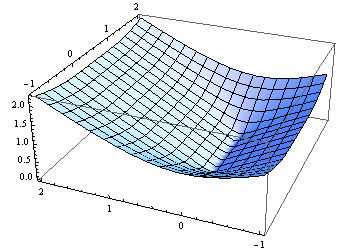
\includegraphics[scale=0.75]{pictures/PtLSplot}
			}
			\caption{Plot of Point to Line Segment Distance}
			\end{figure}

			Theory source: \url{http://math.stackexchange.com/a/322836} \newline
			Code source: \url{http://stackoverflow.com/a/1501725} \newline

\subsection{Testing}

	\definecolor{lightgray}{gray}{0.9}

	\begin{tabular}{| p{2cm} | p{7cm} | p{3cm} |}
		\hline
		\rowcolor{lightgray}
		{\bf Test Case} & {\bf Result} & {\bf Pass/Not pass} \\ \hline

	  	FT-06 Build Power Lines &  &  \\ \hline

	  	FT-11 Collect Money &  &  \\ \hline

	  	FT-14 Win Game &  &  \\ \hline
	  	
	  	FT-16 Limited Power &  &  \\ \hline
	  	
	  	FT-17 Remove Power Cables &  &  \\ \hline
	  	
	  	FT-18 Number of Power Plants &  &  \\ \hline
	  	
	  	FT-19 Different Buildings &  &  \\ \hline

	  	FT-20 Damaged Power Lines &  &  \\ \hline
	  	
	  	FT-21 Enter next level &  &  \\ \hline

	  	FT-22 Appearance of buildings in new levels &  &  \\ \hline

	  	FT-23 More unstable power lines in new levels &  &  \\ \hline

	  	FT-25 Selected houses &  &  \\ \hline

	  	FT-26 Color of power cable &  &  \\ \hline

	\end{tabular}

\subsection{Changes to the requirements}

	As we worked during thi sprint we made some changes to the requirement specification.
	The first is FR 1.2 that we changed priority on. 

	The requirement (FR 6.5) with notification for new obstacles is removed. 
	The group defined a sound as a notification and will discuss within the group if
	we want to have a sound of not, but the visual notification will not be implemented. 

	Since the game is in a state where it is playable we have focused some more on the 
	GUI, and therefore have added some new requirements (FR 1.11 - FR 1.13) that were missing 
	from the specification.
	
	{\bf All changes on version 3 of the requirement specification:} \\
	\begin{tabular}{| p{1.5cm} | p{12cm} |}
		\hline
		\rowcolor{lightgray}
		{\bf FR} & {\bf Change} \\ \hline
		FR 1.2 & {\bf \color{orange}[CHANGED PRIORITY FROM HIGH TO MEDIUM]} The user should be able 
		to exit the game at any time, and the game state should be saved and loaded when the user 
		returns to the game \\ \hline
		FR 4.6 & {\bf \color{green}[NEW]} The user should be able to win the game by reaching the goal in the current level. The goal is level specific. \\ \hline
		FR 6.5 & {\bf \color{red}[REMOVED]} The user shoud get a notification of new events outside 
		the screen \\ \hline
		FR 6.11 & {\bf \color{green}[NEW]} The user should be able to see which houses is selected when building power cables. \\ \hline
		FR 6.12 & {\bf \color{green}[NEW]} The cables should change color if it is connected to a power 
		station. \\ \hline
		FR 6.13 & {\bf \color{green}[NEW]} The user should be able to see how much power the 
		powerplant have left. This bar should decrease if a building is connected to the powerplant 
		and should be increase if a building is removed. The colors should be yellow whit white 
		background. \\ \hline
	\end{tabular}


\subsection{Group dynamics}
	As a group, it is important to have fun. In the start of the project, the group had some
	problems with the communication, but this is not a problem anymore.
	When the group work we talk about what we read on reddit, what we did yesterday and 
	"bully" each other for funny writing typo, if found, in this report. 

	The harmony in the group is now great and it helps us keep up the good work and meet 
	our sprint goals. We belive having fun is the key to succeed in this project. 

\subsection{Customer feedback}

\subsection{Sprint retrospective}
	In this sprint, we did not do the sprint retrospective, but all the team members did
	get the chance to add changes to the next and last sprint. We are quite pleased with the way 
	we work and non of the group members had anything specific to add or remove in the next sprint.

	We have only had one situation where two of the team members worked on the same implementation, 
	but we dont think that would happend again and have not been a problem up until now. 
	The group need to ensure a good communication within the group as well as give good status
	updates while working. 

	The group agreed to keep up the good work. "Team spirit!".
